
\section{Sobre nuestro código programado en Ruby}

\subsection{Lenguaje de programación Ruby}

Ruby es un lenguaje con un balance cuidado. Su creador, Yukihiro ''Matz'' Matsumoto, mezcló partes de sus lenguajes favoritos (Perl, Smalltalk, Eiffel, Ada, y Lisp) para formar un nuevo lenguaje que incorporara tanto la programación funcional como la programación imperativa.

A menudo ha manifestado que está ''\em{tratando de hacer que Ruby sea natural, no simple}'', de una forma que se asemeje a la vida real.\\
Continuando sobre esto, agrega: \em{Ruby es simple en apariencia, pero complejo por dentro, como el cuerpo humano}.

Ruby tiene un conjunto de otras funcionalidades entre las que se encuentran las siguientes:

\begin{itemize}
\item Manejo de excepciones, como Java y Python, para facilitar el manejo de errores.
\item Un verdadero mark-and-sweep garbage collector para todos los objetos de Ruby. No es necesario mantener contadores de referencias en bibliotecas externas. Como dice Matz, “Esto es mejor para tu salud”.
\item Escribir extensiones en C para Ruby es más fácil que hacer lo mismo para Perl o Python, con una API muy elegante para utilizar Ruby desde C. Esto incluye llamadas para embeber Ruby en otros programas, y así usarlo como lenguaje de scripting. También está disponible una interfaz SWIG.
\item Puede cargar bibliotecas de extensión dinámicamente si lo permite el sistema operativo.
\item Tiene manejo de hilos (threading) independiente del sistema operativo. De esta forma, tienes soporte multi-hilo en todas las plataformas en las que corre Ruby, sin importar si el sistema operativo lo soporta o no, ¡incluso en MS-DOS!
\item Ruby es fácilmente portable: se desarrolla mayoritariamente en GNU/Linux, pero corre en varios tipos de UNIX, Mac OS X, Windows 95/98/Me/NT/2000/XP, DOS, BeOS, OS/2, etc.
\item Al ser un lenguaje moderno, maneja cantidades numéricas estratosfericas.
\end{itemize}




\subsection{Sobre el entorno de desarrollo}

Sobre el IDE utilizado:
\begin{itemize}
\item Nombre del IDE: Aptana Studio 3
\item Link de descarga del IDE: \url{http://aptana.com/products/studio3}
\item Descripción del IDE: Aptana Studio 3 es una herramienta de desarrollo profesional de código abierto para la web abierta. Su principal función es desarrollar y probar la aplicación web completa utilizando un único entorno. Con soporte para las últimas especificaciones de tecnología del navegador, como HTML5, CSS3, JavaScript, Ruby, Rails, PHP y Python.
\begin{figure}[h]
\centering
    
\includegraphics[width=8cm]{aptana-logo.png}
\end{figure}
\end{itemize}

Sobre el lenguaje de programación utilizado:
\begin{itemize}
\item Nombre del lenguaje: Ruby, versión 1.9.3
\item Link de descarga: \url{https://www.ruby-lang.org/en/downloads/}
\end{itemize}

Sobre el código implementado para representar la búsqueda binaria recursiva, podemos resumir las siguientes características:
\begin{itemize}
\item Una única clase con sus inherentes métodos
\item Métodos que permiten fácil manipulación y entendimiento del código
\item Variables Nemotécnicas
\end{itemize}

Sobre el codigo en sí:
\begin{itemize}
\item Búsqueda binaria recursiva
\item Estructura utilizada: Un arreglo de largo $N$
\begin{figure}[h]
\centering
    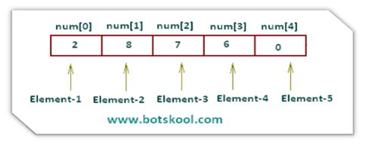
\includegraphics[width=10cm]{imagen_1.png}
\end{figure}
\item Permite distintos poblamientos de los datos:
\begin{itemize}
\item Ordenado automático (de entrada sin usar ordenamiento burbuja)
\item Aleatorio
\item Manual
\end{itemize}
\begin{figure}[H]
\centering
    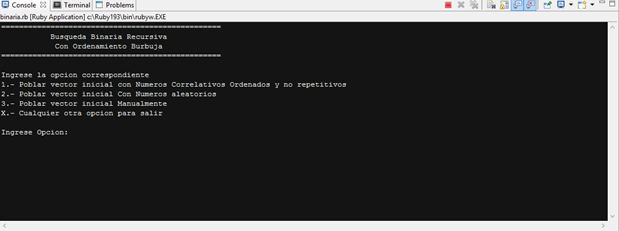
\includegraphics[width=\textwidth]{imagen_2.png}
\end{figure}

\item Fácil Manipulación del Código

Al ser un programa escrito a modo de ejemplo se intentó hacer lo más simple de manipular posible, con tal de alguna vez aplicarlo en algún problema real. Se documentó muy en extenso el código y se identó de tal forma que para cualquier programador, por inexperto que sea podrá manipular el código. 

Se abusó del uso de métodos para que la comprensión y manipulación del código fuera la más fidedigna posible, resultando seguro, fiable, robusto, usable y portable.

\item Método de Ordenamiento Burbuja (alternativo)

El algoritmo de ordenación por el método de la burbuja, también conocido como intercambio directo, es uno de los más simples que se conocen. Se basa en una serie de intercambios entre elementos adyacentes. Esos intercambios dan la impresión de que cada elemento va ascendiendo a través del array acercándose cada vez más a su posición final, recordando a cómo ascienden las burbujas de gas en un líquido.

A efectos prácticos, el algoritmo de la burbuja no es adecuado prácticamente para ninguna situación, ya que realiza muchas comparaciones y muchos intercambios. Pero para efectos prácticos solo se usa este algoritmo para demostrar la dependencia de datos ordenados en la búsqueda binaria recursiva. Hay algoritmos similares que se comportan bastante mejor pero su interés es más bien teórico, ya que sirve para establecer comparativas con otros métodos y extraer conclusiones teóricas.

\begin{figure}[H]
\centering
    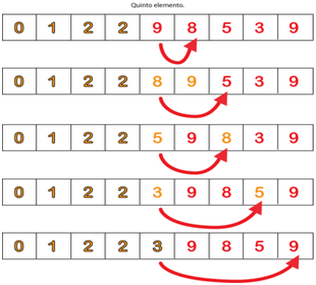
\includegraphics[width=8cm]{imagen_3.png}
\end{figure}

\end{itemize}

\newpage
\subsection{Código en Ruby}

%%%%%%%%%%%%%%%%%%%%%%%%%%%%%%%%%%%%%%%%%%%%
%%%%%%%%%%%%%%%%%%%%%%%%%%%%%%%%%%%%%%%%%%%%

{
\ttfamily \scriptsize



\noindent \#programa: Busqueda Binaria Recursiva

\bigskip 
\noindent require 'date'

\noindent require 'Time'

\bigskip 
\noindent class Bbinario

\bigskip 
\noindent \ \   \#Variables de la clase

\noindent \ \   @@operaciones = 0  

\noindent \ \   @@tiemporFinalBusqueda = 0.00000000

\noindent \ \   @@tiemporFinalOrdenamiento = 0.00000000

\noindent \ \   \#Llena el vector inicial manualmente

\noindent \ \   def self.llenarManualmente(vector, num)

\noindent \ \ \ \ \ \       i = 0

\noindent \ \ \ \ \ \       loop do

\noindent \ \ \ \ \ \ \ \ \          puts "Ingrese Numero \#\{i\}"

\noindent \ \ \ \ \ \ \ \ \          vector[i] = gets.chomp.to\_i

\noindent \ \ \ \ \ \ \ \ \          return vector if i == num

\noindent \ \ \ \ \ \ \ \ \          i=i+1

\noindent \ \ \ \ \ \       end

\noindent \ \   end

\bigskip 
\noindent \ \   \#Llenar aleatoriamente

\noindent \ \   def self.llenarAleatorio(vector, num)

\bigskip
\noindent \ \ \ \ \ \       i = 0      

\noindent \ \ \ \ \ \       loop do         

\noindent \ \ \ \ \ \ \ \ \          vector[i] = rand(999) + 1

\noindent \ \ \ \ \ \ \ \ \          return vector if i == num

\noindent \ \ \ \ \ \ \ \ \          i=i+1

\noindent \ \ \ \ \ \       end

\noindent \ \   end

\bigskip 
\noindent \ \   \#Llenar en Orden no repetidos

\noindent \ \   def self.llenarNoRepetidos(vector, num)

\bigskip
\noindent \ \ \ \ \ \       i = 0

\noindent \ \ \ \ \ \       loop do         

\noindent \ \ \ \ \ \ \ \ \          vector[i] = i

\noindent \ \ \ \ \ \ \ \ \          i=i+1

\noindent \ \ \ \ \ \ \ \ \          return vector if i == num

\bigskip 
\noindent \ \ \ \ \ \       end

\noindent \ \   end

\bigskip 
\noindent \# metodo de ordenamiento burbuja

\noindent \ \   def self.ordenar(vector)

\noindent \ \ \ \     inicio = Time.now

\noindent \ \ \ \ \ \       for i in 0..vector.length-2

\noindent \ \ \ \ \ \ \ \ \          for j in i+1...vector.length

\noindent \ \ \ \ \ \ \ \ \ \ \ \ \              if vector[i] > vector[j]

\noindent \ \ \ \ \ \ \ \ \ \ \ \ \ \ \ \                 aux = vector[j]

\noindent \ \ \ \ \ \ \ \ \ \ \ \ \ \ \ \                 vector[j] = vector[i]

\noindent \ \ \ \ \ \ \ \ \ \ \ \ \ \ \ \                 vector[i] = aux

\noindent \ \ \ \ \ \ \ \ \ \ \ \ \              end

\noindent \ \ \ \ \ \ \ \ \          end

\noindent \ \ \ \ \ \       end      

\noindent \ \ \ \ \ \       termino = Time.now

\noindent \ \ \ \ \ \       @@tiemporFinalOrdenamiento = termino - inicio

\noindent \ \ \ \ \ \       return vector

\noindent \ \   end

\bigskip 
\noindent \ \   \#Mostrar en pantalla el vector generado y ordenado

\noindent \ \   def self.imprimir(vector)

\noindent \ \ \ \ \ \       vector.each do |i|

\noindent \ \ \ \ \ \ \ \ \          print "|\#\{i\}"

\noindent \ \ \ \ \ \       end

\noindent \ \ \ \ \ \       print "|"

\noindent \ \   end

\bigskip 
\noindent \ \   \# Se define la cantidad de entrada en el arreglo

\noindent \ \   def self.getCantidad

\noindent \ \ \ \     print "Ingrese Cantidad de Datos en el arreglo inicial: "

\noindent \ \ \ \     STDOUT.flush

\noindent \ \ \ \     cant = gets.chomp.to\_i

\noindent \ \ \ \     return cant

\noindent \ \   end   

\bigskip 
\noindent \ \   \# Se obtiene el valor a encontrar

\noindent \ \   def self.getBuscado

\noindent \ \ \ \     print "	extbackslashn	extbackslashnIngrese el numero a buscar: "

\noindent \ \ \ \     STDOUT.flush

\noindent \ \ \ \     cant = gets.chomp.to\_i

\noindent \ \ \ \     return cant

\noindent \ \   end   

\bigskip 
\noindent \ \   \# Algoritmo de busqueda binaria recursiva

\noindent \ \   def self.busquedaBinariaRecursiva(vector, val, left, right)

\bigskip 
\noindent \ \ \ \     if (left + right) \% 2 == 0

\noindent \ \ \ \ \ \       mid = (left + right) / 2 

\noindent \ \ \ \     else

\noindent \ \ \ \ \ \ \        mid = (left + right) / 2  + 1 

\noindent \ \ \ \     end

\noindent \ \ \ \     return -999 if left > right

\bigskip 
\noindent \ \ \ \     @@operaciones = @@operaciones + 1;

\bigskip 
\noindent \ \ \ \     if val == vector[mid]

\noindent \ \ \ \ \ \       return mid 

\noindent \ \ \ \     elsif val > vector[mid]

\noindent \ \ \ \ \ \       busquedaBinariaRecursiva(vector, val, mid + 1, right)

\noindent \ \ \ \     else

\noindent \ \ \ \ \ \       busquedaBinariaRecursiva(vector, val, left, mid - 1)

\noindent \ \ \ \     end

\noindent \ \   end

\bigskip 
\noindent \ \   \#Funcion donde se defie como y donde aplicar el algoritmo, con las condiciones entregadas por parametro

\noindent \ \   def self.aplicarAlgoritmo(arreglo, cant)

\noindent \ \ \ \     inicio = Time.now.to\_f 

\noindent \ \ \ \     \#ordenar(arreglo)

\noindent \ \ \ \     termino = Time.now.to\_f

\noindent \ \ \ \     print "	extbackslashn	extbackslashnEl tiempo total empleado en el ordenamiento fue: "    

\noindent \ \ \ \     orden = termino - inicio

\noindent \ \ \ \     print  "\%.7f Segundos" \%(termino - inicio) 

\bigskip 
\noindent \ \ \ \     \#Para numeros grandes deshabilitar mostrar el vector ordenado

\noindent \ \ \ \     puts "	extbackslashnEl vector ingresado y ordenado fue"    

\noindent \ \ \ \     \#imprimir(arreglo)    

\bigskip 
\noindent \ \ \ \     buscado = getBuscado

\noindent \ \ \ \     inicioU = Time.now.to\_f 

\noindent \ \ \ \     sleep(0.1)

\noindent \ \ \ \     nuevo = busquedaBinariaRecursiva(arreglo,buscado,0,cant-1)

\noindent \ \ \ \     terminoU = Time.now.to\_f    

\noindent \ \ \ \     busqueda = termino - inicio

\noindent \ \ \ \     if nuevo == - 999

\noindent \ \ \ \ \ \       puts "No se encontro el valor buscado, por lo tanto es el peor caso a evaluar"     

\noindent \ \ \ \ \ \       print "	extbackslashn	extbackslashnLa cantidad de operaciones necesarias fueron: "

\noindent \ \ \ \ \ \       print @@operaciones  

\noindent \ \ \ \ \ \       print "	extbackslashn	extbackslashnEl tiempo de ejecucion total en la busqueda fue: "    

\noindent \ \ \ \ \ \       print  "\%.7f Segundos" \%(terminoU - inicioU - 0.1)

\noindent \ \ \ \ \ \       print "	extbackslashn	extbackslashnEl tiempo total empleado en la ejecucion: "    

\noindent \ \ \ \ \ \       print  "\%.7f Segundos" \%((termino - inicio) + (terminoU - inicioU - 0.1))   

\bigskip 
\noindent \ \ \ \     else

\noindent \ \ \ \ \ \       print "	extbackslashnLa posicion del valor buscado en el arreglo inicial es: "

\noindent \ \ \ \ \ \       print nuevo + 1

\noindent \ \ \ \ \ \       print "	extbackslashn	extbackslashnLa cantidad de operaciones necesarias fueron: "

\noindent \ \ \ \ \ \       print @@operaciones  

\noindent \ \ \ \ \ \       print "	extbackslashn	extbackslashnEl tiempo total empleado en la busqueda fue: "    

\noindent \ \ \ \ \ \       print  "\%.7f Segundos" \%(terminoU - inicioU - 0.1) 

\noindent \ \ \ \ \ \       print "	extbackslashn	extbackslashnEl tiempo total empleado en la ejecucion: "    

\noindent \ \ \ \ \ \       print  "\%.7f Segundos" \%((termino - inicio) + (terminoU - inicioU - 0.1))      

\noindent \ \ \ \     end

\noindent \ \   end

\bigskip 
\noindent \ \   \# Funcion pricipal para ejecutar donde se definen los datos de entrada

\noindent \ \   def self.principal

\noindent \ \ \ \ \ \       arregloInicial = Array.new

\noindent \ \ \ \ \ \       operacion = 0

\noindent \ \ \ \ \ \       puts "================================================="

\noindent \ \ \ \ \ \       puts "           Busqueda Binaria Recursiva"

\noindent \ \ \ \ \ \       puts "            Con Ordenamiento Burbuja"

\noindent \ \ \ \ \ \       puts "================================================="

\noindent \ \ \ \ \ \       puts " "

\noindent \ \ \ \ \ \       puts "Ingrese la opcion correspondiente"

\noindent \ \ \ \ \ \       puts "1.- Poblar vector inicial con Numeros Correlativos Ordenados y no repetitivos"

\noindent \ \ \ \ \ \       puts "2.- Poblar vector inicial Con Numeros aleatorios"

\noindent \ \ \ \ \ \       puts "3.- Poblar vector inicial Manualmente "

\noindent \ \ \ \ \ \       puts "X.- Cualquier otra opcion para salir"

\noindent \ \ \ \ \ \       puts " "

\noindent \ \ \ \ \ \       print "Ingrese Opcion: "

\noindent \ \ \ \ \ \       STDOUT.flush

\noindent \ \ \ \ \ \       opcion = gets.chomp.to\_i

\noindent \ \ \ \ \ \       if opcion == 1

\noindent \ \ \ \ \ \ \ \         puts "Se poblara con Numeros Correlativos, no repetitivos"

\noindent \ \ \ \ \ \ \ \         cantidad = getCantidad

\noindent \ \ \ \ \ \ \ \         llenarNoRepetidos(arregloInicial, cantidad)

\noindent \ \ \ \ \ \ \ \         aplicarAlgoritmo(arregloInicial, cantidad)

\bigskip 
\noindent \ \ \ \ \ \       elsif opcion == 2

\noindent \ \ \ \ \ \ \ \         puts "Se poblara Con Numeros aleatorios"

\noindent \ \ \ \ \ \ \ \         cantidad = getCantidad

\noindent \ \ \ \ \ \ \ \         llenarAleatorio(arregloInicial, cantidad)        

\noindent \ \ \ \ \ \ \ \         aplicarAlgoritmo(arregloInicial, cantidad)

\bigskip 
\noindent \ \ \ \ \ \       elsif opcion == 3

\noindent \ \ \ \ \ \ \ \       puts "Se poblara Manualmente"

\noindent \ \ \ \ \ \ \ \       cantidad = getCantidad

\noindent \ \ \ \ \ \ \ \       llenarManualmente(arregloInicial, cantidad)

\noindent \ \ \ \ \ \ \ \       aplicarAlgoritmo(arregloInicial, cantidad)

\bigskip 
\noindent \ \ \ \ \ \       else 

\noindent \ \ \ \ \ \ \ \         puts "Se ingreso la Opcion Salir del Programa"

\noindent \ \ \ \ \ \ \ \         puts "Programado en Ruby V 1.9.3"

\noindent \ \ \ \ \ \ \ \         puts "Juan Cid Carrenio"

\noindent \ \ \ \ \ \ \ \         puts "Manuel Irarrazabal"

\noindent \ \ \ \ \ \ \ \         puts "Rafael Vivar"

\noindent \ \ \ \ \ \ \ \         puts "Daniel Gutierrez"

\noindent \ \ \ \ \ \ \ \         puts "Grupo Alias"

\noindent \ \ \ \ \ \       end

\noindent \ \   end

\bigskip 
\noindent end

\bigskip 
\noindent Bbinario.principal



}

%%%%%%%%%%%%%%%%%%%%%%%%%%%%%%%%%%%%%%%%%%%%
%%%%%%%%%%%%%%%%%%%%%%%%%%%%%%%%%%%%%%%%%%%%

\subsection{Pruebas al programa}

\subsubsection{Peor caso}

\begin{center}
\begin{tabular}{|c|c|}
\hline
\cellcolor[gray]{0.85} \textbf{Número de datos} & 	\cellcolor[gray]{0.85} \textbf{Cantidad de operaciones}\\

\hline
1.000		&	10\\
\hline
10.000	&	14  \\
\hline
100.000	&	17  \\
\hline
1.000.000	&	20  \\
\hline
10.000.000	&	24  \\
\hline
100.000.000	&	27  \\
\hline
\end{tabular}
\end{center}

\subsubsection{Mejor caso}

\begin{center}
\begin{tabular}{|c|c|}
\hline
\cellcolor[gray]{0.85} \textbf{Número de datos} & 	\cellcolor[gray]{0.85} \textbf{Cantidad de operaciones}\\

\hline
1.000		&	1\\
\hline
10.000	&	1  \\
\hline
100.000	&	1  \\
\hline
1.000.000	&	1  \\
\hline
10.000.000	&	1  \\
\hline
100.000.000	&	1  \\
\hline
\end{tabular}
\end{center}

\subsubsection{Ejecución del programa}

\begin{figure}[h]
\centering
    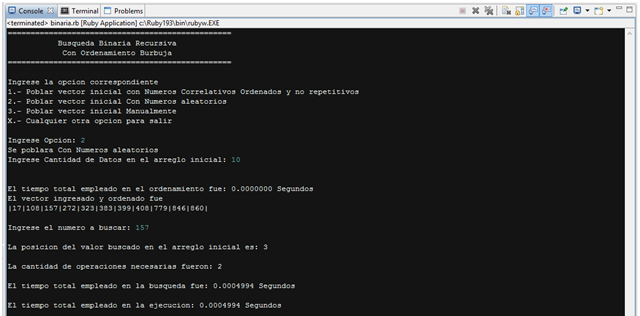
\includegraphics[width=\textwidth]{imagen_4.png}
\end{figure}


